\documentclass[../main.tex]{subfiles}

\begin{document}
\section{Task 1 -- XGBoost}
The model was trained using mostly default parameters of the Python
\verb`xgboost` module. Despite this, it managed to achieve quite tremendous
results, as visible in table \ref{table:perf}.

\subsection{Model visualization}
\begin{figure}[H]
	\centering
	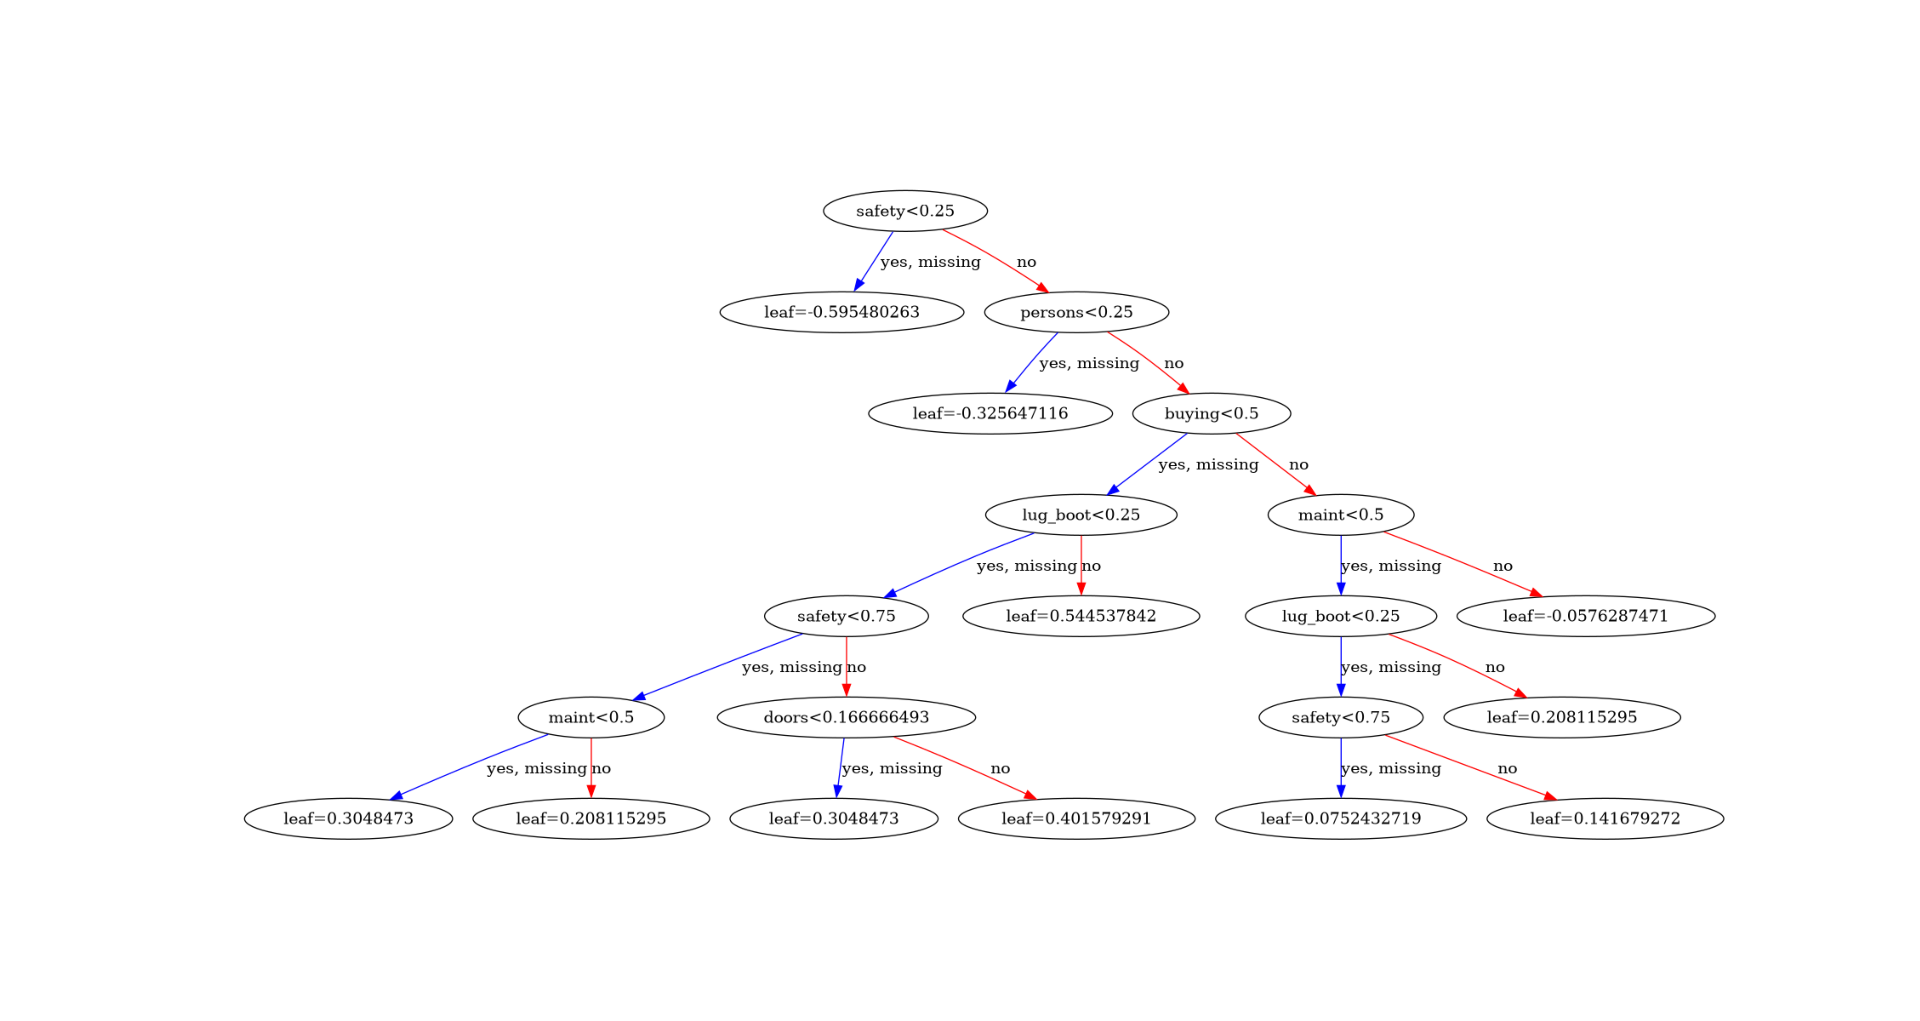
\includegraphics[width=\linewidth]{../img/xgb-tree.png}
	\caption{Last tree in the ensemble produced by XGBoost}
	\label{fig:xgb-tree}
\end{figure}

\subsection{Preference analysis}
% TODO: present DALEX output, comment on it

\paragraph{XGBoost}
The XGBoost library also has native support for quantifying and plotting
feature importance. It must use a slightly different method than DALEX, because
the assigned values and even the ranking of the features are not the same. For
the sake of inter-model comparability, we decided to focus on the DALEX output,
so this next figure is provided only as a curiosity:
\begin{figure}[H]
	\centering
	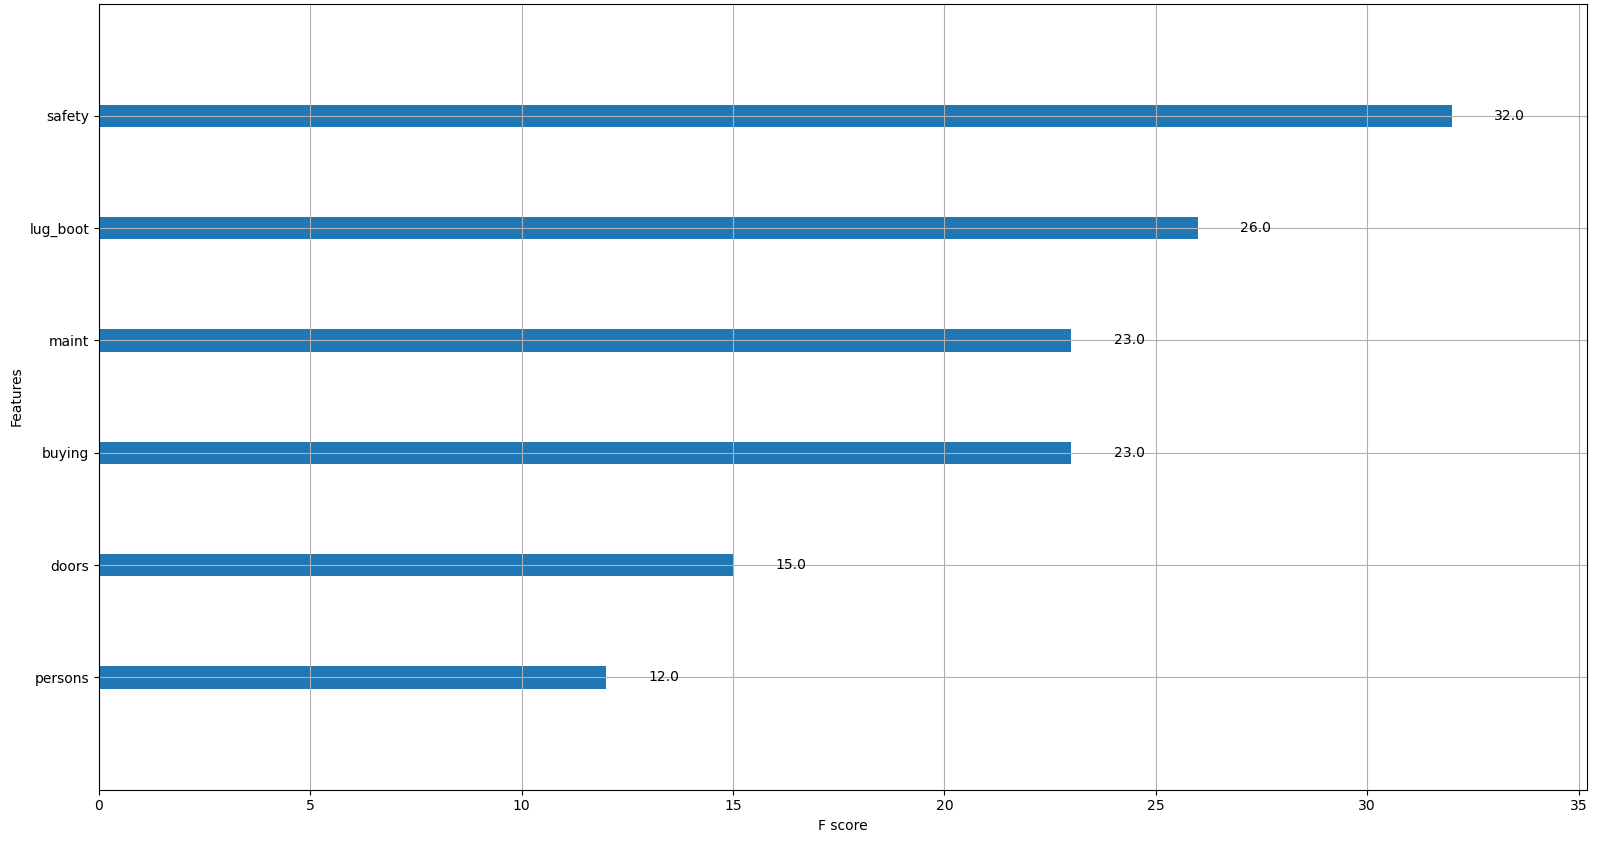
\includegraphics[width=\linewidth]{../img/xgb-feature-importance-xgboost.png}
	\caption{Importance of each feature, according to XGBoost}
	\label{fig:xgb-feats-xgboost}
\end{figure}

\subsection{Remarks}
% TODO

\end{document}
